% !TEX root = Projektdokumentation.tex


\newglossaryentry{Cross-Site-Scripting}{name={Cross-Site-Scripting},description={
		Cross-site scripting (XSS) ist ein Angriff auf eine Webapplikation, die Benutzereingaben nicht sorgfältig überprüft, bevor diese wieder an weitere Benutzer zurückgeschickt werden. So kann ein Angreifer ausführbaren Code mitgeben, der anschliessend bei vielen anderen Benutzern im Browser ausgeführt wird \cite{whatIs_xss}}}

\newglossaryentry{Vulnerability}{name={Vulnerability},description={
		Fehler im Code oder Design, welcher ein potentielles Sicherheitsrisiko darstellt \cite{whatIs_vulnerability}}}

\newacronym{IKF}{IKF}{Institut für Kommunikation \& Führung}

\newacronym{SKMF}{SKMF}{Swiss Knowledge Management Forum}

%Analyse der Aufgabenstellung, Requirements Engineering, Umfeldanalyse (vergleichbare Produkte und Lösungen), Resultate der Literaturrecherche
%Auch: Ziel und Zweck von Mobile Quiz, wofür und vom wem wird es eingesetzt? Was ist zukünftiges Ziel?

% Hier werden alle Erkenntnisse aus den einzelnen Unterkapitel zusammengefasst.
%ohne Titel

%Hier noch eine Zusammenfassung
Um ein möglichst gutes Bild davon zu erhalten, was im Bereich Online-Quizzes bereits vorhanden ist und wo Mobile Quiz aktuell steht, wurden Informationen in verschiedenen Bereichen gesucht und zusammengetragen.

Dazu wurden unter anderem ähnliche Arbeiten, im Sinne von Bachelorarbeiten oder Studienarbeiten, gesucht (Punkt \ref{sec:eigeneUntersuchungenWebuntersuchungen}) und diese auf ihre Relevanz überprüft. Dabei wurde festgestellt, dass sich, was Arbeiten von Studierenden betrifft, vor allem die HSR auf Quizzes im Lernbereich konzentriert.
Das Testen von Mobile Quiz selbst (Punkt \ref{subsec:eigeneUntersuchungen}) zeigte, dass es noch einige Probleme in der Version 3 anzutreffen gab. Diese zu beheben würde die Plattform solider machen und bestenfalls neue Quiz-Ersteller anziehen.
Weiter wurde beim Vergleich mit anderen Online-Quiz-Plattformen (Punkt \ref{subsec:Webuntersuchungen}) ersichtlich, dass Mobile Quiz im Bereich Funktionsumfang und Einstellungsmöglichkeiten gut dastand. Allerdings konnte das Mobile Quiz im Bereich Usability nicht Punkten, da viele Funktionen nicht sofort ersichtlich oder nur schwierig zu erreichen waren. Dies wurde auch durch die Usability-Tests (Abschnitt \ref{sec:usability}) bestätigt, welche ebenfalls zu Beginn der Arbeit durchgeführt wurden.

Die Ergebnisse aus dieser Untersuchung flossen zusammen mit den bereits bekannten Verbesserungspunkten in die Aufgabenstellung dieser Studienarbeit ein. Diese ist im Anhang unter 'MoeglicheArbeitenSA.pdf' ersichtlich. Um nicht jeden Bug einzeln aufzuführen, wurden darin die Probleme abstrahiert und nur Themenbereiche aufgeführt und beschrieben. Diese wurden besprochen und nach ihrer Wichtigkeit priorisiert.

\newpage

\section{Recherche/ähnliche Arbeiten}

Welche ähnlichen Arbeiten, seien es Bachelorarbeiten, Studienarbeiten oder sonstige Arbeiten in ähnlichem Umfang, gibt es bereits?

Da es kein zentrales, Schulen übergreifendes Verzeichnis aller Arbeiten gibt, musste zur Beantwortung dieser Frage die einzelnen Verzeichnisse der Schulen durchgegangen werden. Dabei wurden die folgende Schulen, aufgelistet mit dem jeweiligen gefundenen Ergebnissen, beachtet:
\begin{itemize}
	\item ETH Zürich
	\begin{itemize}
		\item Die Arbeiten, welche an der ETH Zürich erstellt wurden, behandeln spezifisch auf die Prüfungssituation ausgelegte Tools. Diese Arbeiten wurden deshalb nicht weiter im Detail betrachtet. \cite{zeller_automated_2014} \cite{antonucci_autoteach_2014} \cite{heinrich_design_2008} \cite{nanzer_einsatz_2005}
	\end{itemize}
	\item ZHAW
	\begin{itemize}
		\item Im Verzeichnis aller Arbeiten stach die Arbeit \glqq Edu4u. Geschäftsmodell einer Webplattform im E-Learning-Bereich für E-Lectures, Online-Kurse und Filmdokumentationen\grqq heraus. Leider konnte diese Arbeit nicht genauer angeschaut werden, da sie als vertraulich klassifiziert wurde. \cite{_bachelorarbeiten-2013-zhaw-sml.pdf_}
	\end{itemize}
	\item Universität Zürich
	\begin{itemize}
		\item Hier wurde leider kein Verzeichnis der Arbeiten gefunden.
	\end{itemize}
	\item HSR
	\begin{itemize}
		\item Studienarbeiten Crowdsourced Quizzes \cite{_technischer_bericht-quizzenger_crowdsourced_quizzes.pdf_} und Crowdsourced Quizzes 2 \cite{_technischer_bericht-quizzenger-2.pdf_} aus den Jahren 2014 und 2015 jeweils mit Prof. Frank Kock als Betreuer. Als Ergebnis entstand der Quizzenger.
		\item Bachelorarbeit MobileQuiz \cite{khalid_bachelorarbeit_mobile_quiz_juni_2012.pdf_2012} aus dem Jahr 2012 mit Prof. Dr. Peter Heinzmann. Dabei handelt es sich um die Vorgängerarbeit zu unserer Studienarbeit.
		\item Bachelorarbeit Digital Native Quiz \cite{grob_digital_2010} aus dem Jahr 2010, ebenfalls betreut durch Prof. Dr. Peter Heinzmann.
	\end{itemize}
\end{itemize}

Bei der Suche nach ähnlichen Arbeiten, wurde auch der Standard \glqq IMS Question \& Test Interoperability\grqq \cite{imsglobal.org} der IMS Global Learning Consortium entdeckt. Dieser Standard beinhaltet eine umfassende Übersicht von möglichen Fragetypen.

Das IMS Global Learning Consortium setzt sich allgemein dafür ein, dass ein gemeinsamer Standard entsteht, um für Interoperabilität zwischen einzelnen Lernseiten zu sorgen. Bei vertieften Abklärungen wurde festgestellt, dass sowohl Moodle als auch TAO (zwei der Open Source Seiten, welche in der Webuntersuchung angeschaut wurden) sich auf die Standards von IMS Global Learning Consortium ausrichten.

Es wurde entschieden nicht auf die Standards von IMS Global zu wechseln, da es sich um einen zu grossen Aufwand handeln würde. Und weil sich das MobileQuiz nicht auf absehbarer Zeit mit anderen Seiten austauschen wird.


\section{Eigene Untersuchungen, Webuntersuchung}
\label{sec:eigeneUntersuchungenWebuntersuchungen}

Was kann Mobile Quiz heute bereits, wo gibt es noch Probleme und wo steht das Quiz heute im Vergleich zu ähnlichen Webanwendungen? Diese Fragen waren Kern der eigenen Untersuchungen. Einerseits wurde dazu Mobile Quiz selbst intensiv getestet, andererseits wurden mehrere vergleichbare Online-Quizzes gesucht und diese anhand von vorher definierten Kriterien verglichen.


	\subsection{Untersuchung www.mobilequiz.ch}
	\label{subsec:eigeneUntersuchungen}
	Während mehrerer Stunden wurden sowohl in der Rolle als Lernender, welcher ein Quiz nutzt und in der Rolle als Ersteller, welcher ein neues Quiz erstellt die vorhandenen Funktionen ausprobiert. Dabei kamen verschiedene Probleme zutage, die sich grob in die folgenden Kategorien unterteilen lassen:
	
	
	\begin{itemize}
		\item Sicherheitsrelevante Probleme \\
		Dabei handelt es sich um sämtliche Probleme, welche Auswirkungen auf die Sicherheit haben, also die Sicherheit verringern.
		\textit{Beispiel}: Wird eine Frage erfasst, so kann im Fragetext mittels HTML-Script-Tag JavaScript hinterlegt werden, welches beim Anzeigen der Frage beim Teilnehmer ausgeführt wird. Somit hat Mobile Quiz gegenüber Frage-Erstellern eine \gls{Cross-Site-Scripting} - \gls{Vulnerability}. Diese kann ausgenutzt werden, um das Session-Cookie eines Benutzers zu stehlen. Dabei handelt es sich um ein grosses Risiko, denn sobald ein Angreifer das Session-Cookie eines Benutzers hat, kann er sich als diesen Benutzer ausgeben. Worst-Case Szenario für das Mobile Quiz ist, dass sich jemand an der Prüfung als ein anderer Benutzer ausgibt, oder einem anderen Benutzer dazwischenfunkt.
		\item Usability \\
		In dieser Kategorie wurden die Probleme mit der Navigation und dem Auffinden von Funktionen zusammengefasst.
		\textit{Beispiel}: In der Lernkontrollen-Übersicht ist der Start-Button zu wenig ersichtlich.
		\item Probleme/Bugs \\
		In dieser Kategorie wurden alle Fehler und Probleme festgehalten, welche nicht einer spezifischeren Kategorie zugeordnet werden konnte.
		\textit{Beispiel}: Wird bei einer Lernkontrolle festgelegt, dass sie keinen Endzeitpunkt hat, so soll auch kein Enddatum angezeigt werden.
		\item Mobile-Probleme \\
		Hier wurden sämtliche Mobile-spezifischen Probleme festgehalten.
		\textit{Beispiel}: Der Zugriff via Smartphone auf den Profilbereich funktioniert nicht.
		\item Allgemeine Fragen zum Konzept \\
		\textit{Beispiel}: Muss bei einer Registrierung wirklich die Adresse angegeben werden?
		\item Schreibfehler/Grammatik \\
		\textit{Beispiel}: Der Benutzer wird wird teilweise mit 'Sie' angesprochen, andernorts wird die 'Du'-Form verwendet.
	\end{itemize}

	Die ausführlichen Resultate sind im Dokument 'Ergebnisse eigene Tests.pdf' ersichtlich.
	

	\subsection{Vergleich Online-Quizzes}
	\label{subsec:Webuntersuchungen}
	Um andere Online-Quizzes mit Mobile Quiz zu vergleichen mussten zuerst die Kriterien festgelegt werden. Als Grundlage diente eine Excel-Tabelle von Khalid Abdul und Patrik Naef, welche an die Bedürfnisse dieser Arbeit angepasst wurde. Es wurden folgende Vergleichskriterien festgelegt für den Vergleich verschiedener Online-Quizzes:
	\begin{itemize}
		\item Fragemöglichkeiten
		\item Antwortmöglichkeiten
		\item Zeitsteuerung
		\item Visuelle Signale
		\item Fragenauflösung
		\item Testfunktion
		\item Textdarstellung
		\item Auswertungsmöglichkeiten
		\item Internationalisierung
		\item Erfassen von unterschiedlichen Elementen
		\item Allgemein
		\item Spezielle Funktionen
		\item Benutzerfreundlichkeit
	\end{itemize}
	
	\bigskip
	
	Die zu vergleichenden Websites wurden durch Google-Suchen und Empfehlungen von educatorstechnology.com \cite{educatorstechnology.com} ausgewählt.
		
	Um sicher zu sein, dass die durch uns gewählten Webseiten einen repräsentativen Anteil der Lernquizzes abdeckt, haben wir uns mit Institutionen und Personen in Verbindung gesetzt, welche in diesem Umfeld tätig sind. Um Unterstützung angefragt haben wir bei Switch AAA, dem \acrfull{IKF} und beim \acrfull{SKMF}.
	Leider hatte bei Switch AAA niemand Zeit für uns. Beim \acrshort{IKF} haben Sie selbst keine solche Vergleiche, oder falls etwas vorhanden ist, handelt es sich um Unterrichtsmaterial, welches nicht herausgegeben wird. Das \acrshort{SKMF} konnte nur via ein Webformular kontaktiert werden und hat sich bis am 04.11.2016 noch nicht zurückgemeldet.
	
	\bigskip
	
	Die detaillierte Auswertung ist im Dokument 'SA-Mobile-Quiz\_QuizSysteme-Funktionen-Vergleich-Matrix.xlsx' ersichtlich. Im Folgenden werden die wichtigsten Punkte aus dieser Analyse aufgezeigt. Es wird jeweils die Lösung im aktuellen Mobile Quiz der HSR mit der besten Lösung aus den verschiedenen Vergleichsquizzes präsentiert:
	
	\begin{itemize}
		\item Willkommensseite \\
		Webanwender haben eine riesige Auswahl an Seiten, welche auf ihr Bedürfnis zugeschnitten sind. Sie wenden deshalb nicht viel Zeit auf, um sich über eine einzelne Seite genauer zu informieren. Aus diesem Grund ist der erste Eindruck entscheidend, also eine ansprechende Willkommensseite. \\
		
		\begin{figure}[H]
			\centering
			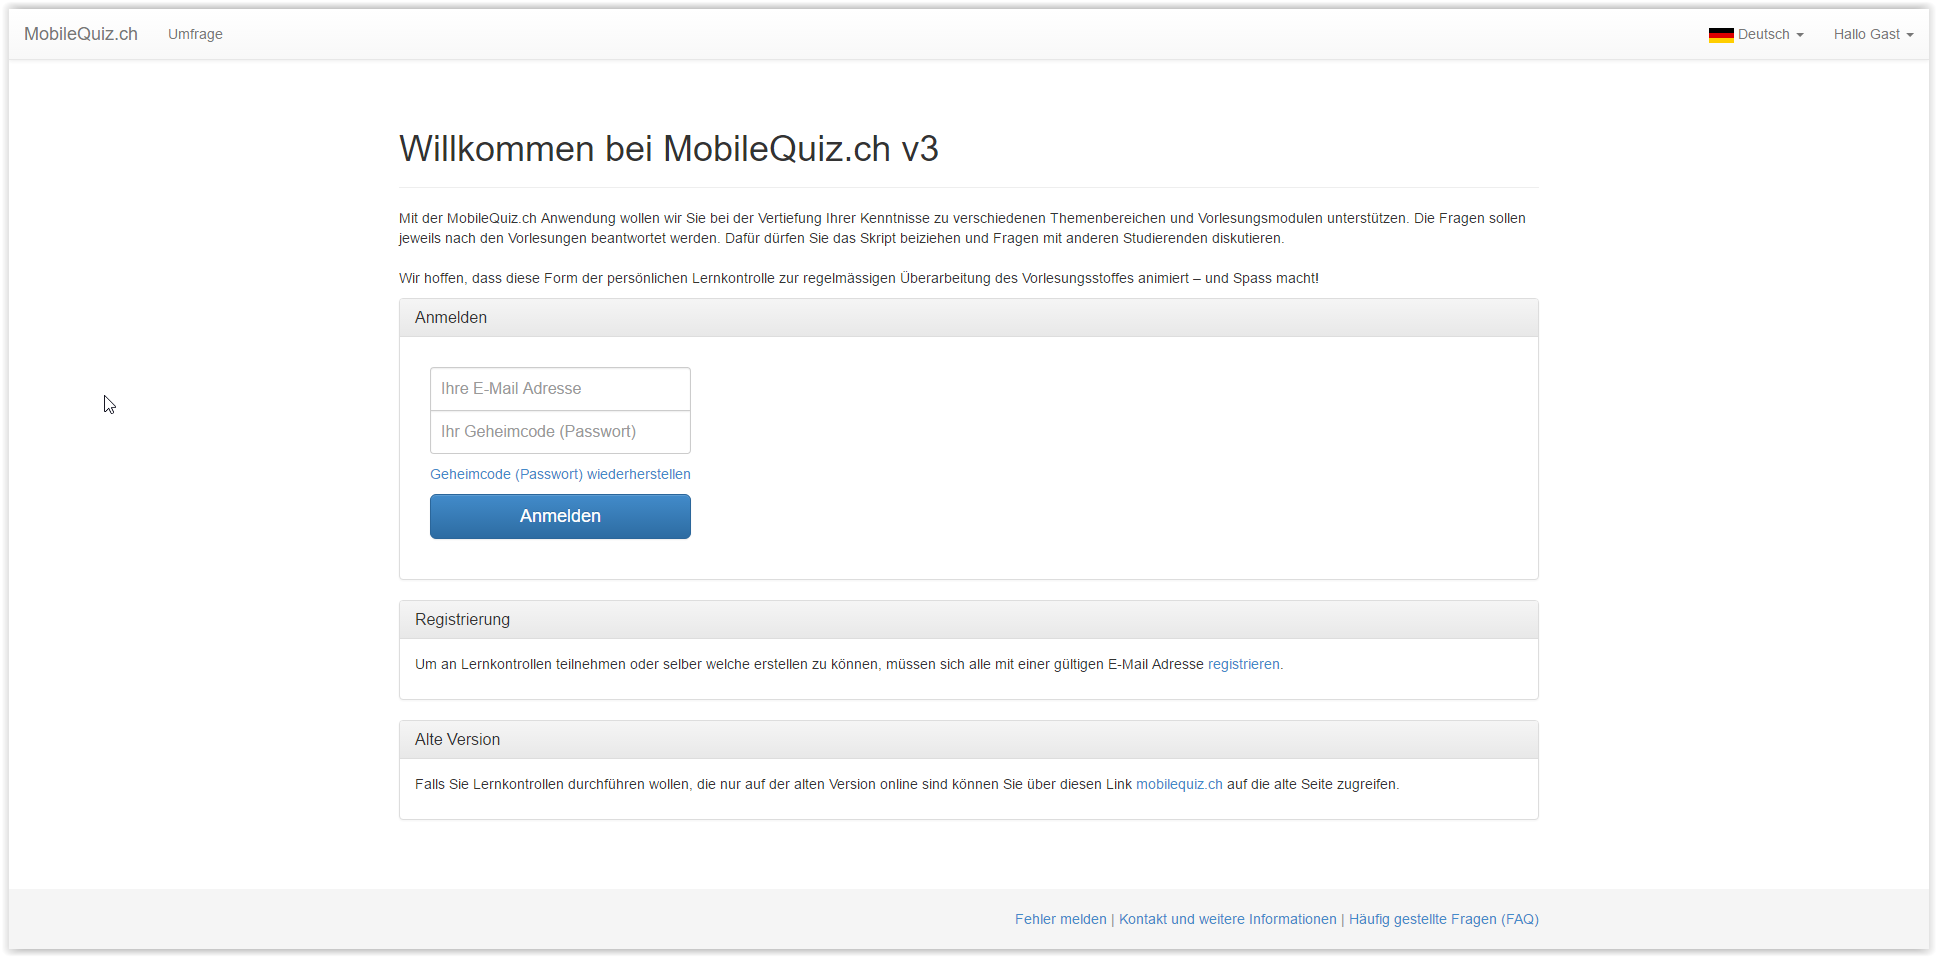
\includegraphics[width=0.75\textwidth]{Images/MobileQuiz_StartPage.PNG}
			\caption{Startseite Mobile Quiz Version 3}
		\end{figure}
		
		Ruft man www.mobilequiz.ch auf, so sieht man viel Text, der die Seite beschreibt. Ein Benutzer weiss jedoch noch nicht genau, was ihn erwartet, wenn er sich registriert und einloggt.
		
		\begin{figure}[H]
			\centering
			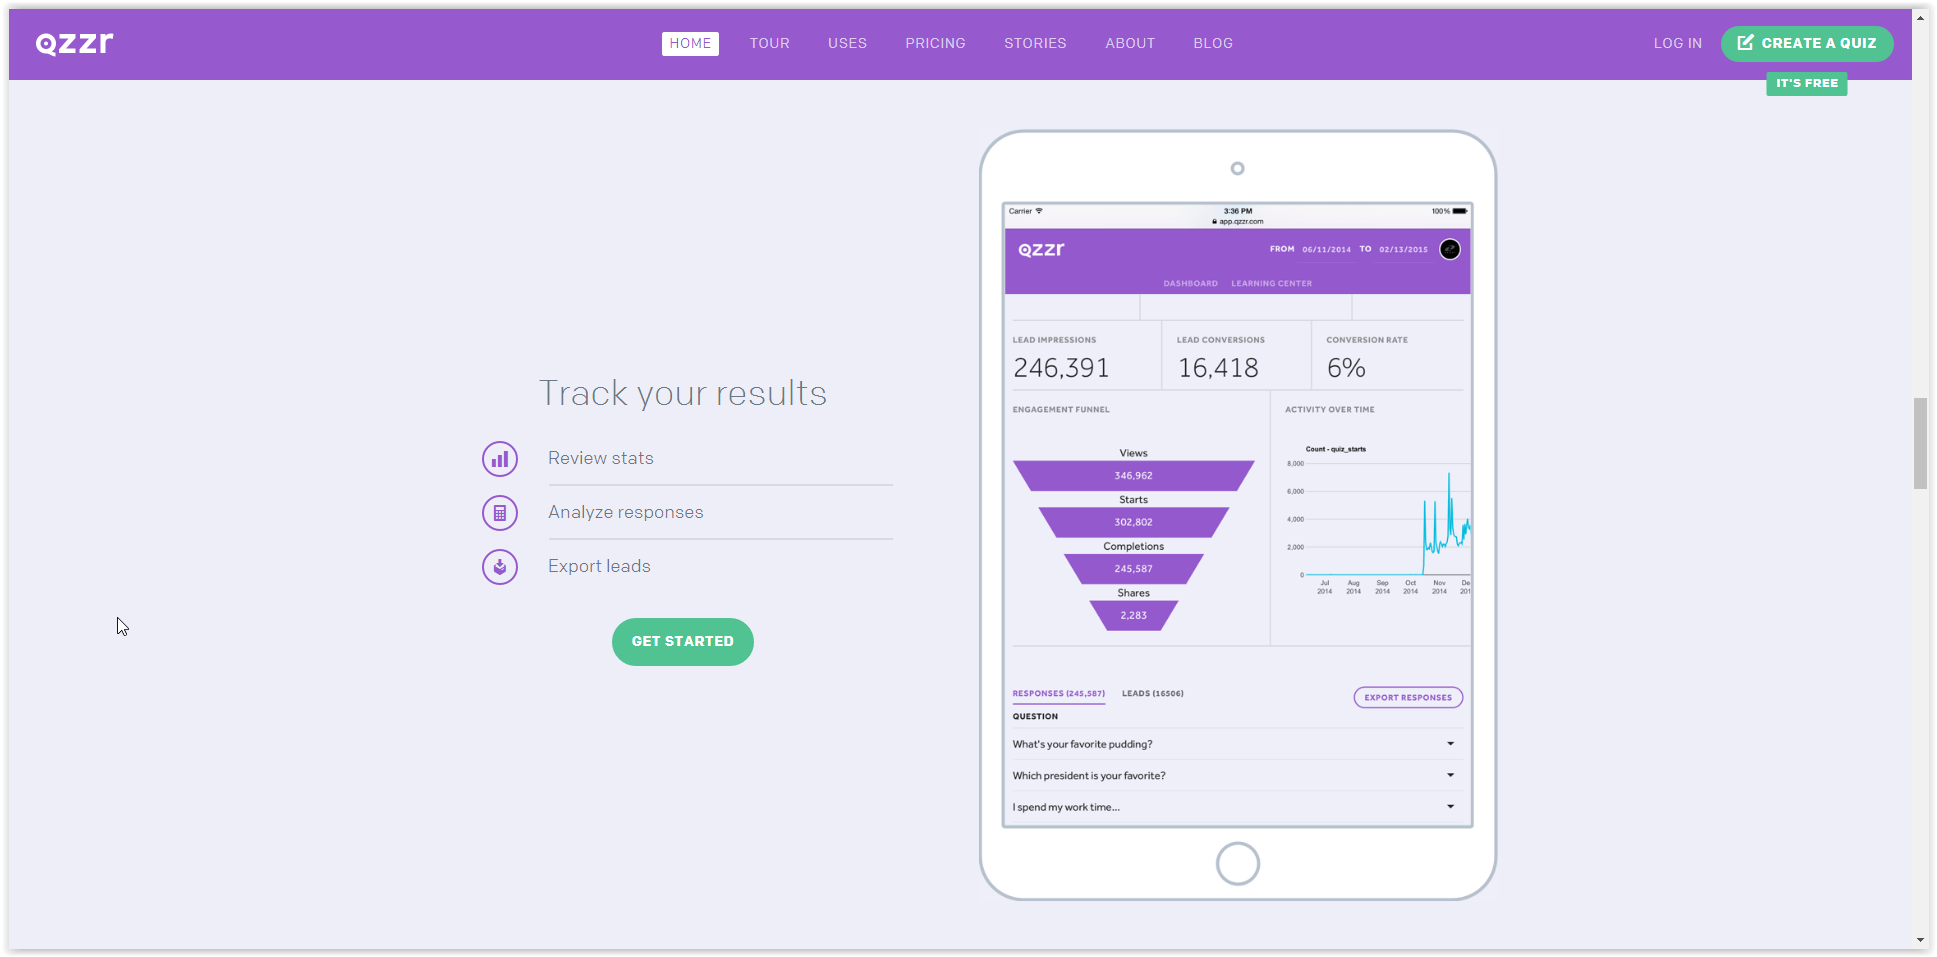
\includegraphics[width=0.75\textwidth]
			{Images/Qzzr_StartPage_Statistics.PNG}
			\caption{Startseite Qzzr}
		\end{figure}
				
		Seiten wie Qzzr \cite{qzzr.com} hingegen, zeigen anhand von Bildern und Symbolen auf, was die Funktionalitäten sind und wie diese konkret aussehen. Solche Bilder sind schnell erfasst  und verarbeitet.
		Mobile Quiz könnte die gleichen Funktionsumfang bieten, aber wenn es der Benutzer nicht sofort sieht, klickt er weiter und registriert sich andernorts.
		
		Was machen gute Willkommensseiten also aus?
		
		\todo{David: Internetrecherche}
		http://blog.hubspot.com/blog/tabid/6307/bid/34006/15-examples-of-brilliant-homepage-design.aspx
		
		
		
		\item Schritt für Schritt - Erstellung von Quizzes \\
		Um ein Quiz zu erstellen benötigt es einerseits die Fragen, andererseits das Quiz selbst, welches mehrere Fragen umfasst. In welcher Reihenfolge sollen diese beiden Ressourcen erstellt werden? \\
		Bei Mobile Quiz war der Ablauf so geregelt, dass zuerst die Fragen und anschliessend das Quiz separat erstellt wurde. War man sich dieser Tatsache bewusst, so stellte dies kein Problem dar, aber war es auch intuitiv? Wie in den durchgeführten Usability-Tests festgestellt wurde, war dem nicht so. Die Benutzer starteten sofort mit der Erstellung des Quizzes, mussten dann aber abbrechen, weil darin keine neuen Fragen erfasst werden konnten.
		Aus diesem Grund war es sinnvoll, diese Reihenfolge in Mobile Quiz zu ändern. Hier bot Testmoz \cite{testmoz.com} ein gutes Vorgehen:
		
		\begin{enumerate}
			\item Testnamen eingeben
			\item Testeinstellungen vornehmen
			\item Fragen erfassen
			\item Veröffentlichen
			\item Reports anschauen
		\end{enumerate}
		
		\begin{figure}[H]
			\centering
			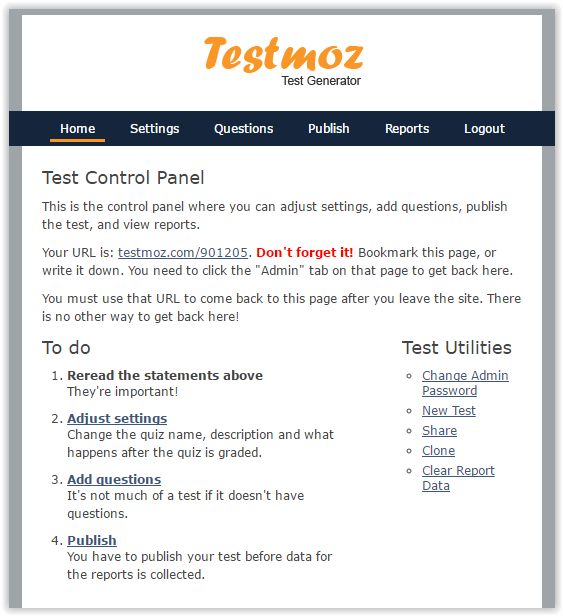
\includegraphics[width=0.4\textwidth]{Images/Testmoz2.PNG}
			\caption{Ablauf Testmoz}
		\end{figure}
		
		Der Ablauf von Mobile Quiz war einzig darin zu ändern, dass neue Fragen während der Erstellung eines Quizzes erfasst werden können. Zur Vereinfachung konnte auch beitragen, dass der Ablauf wie bei Testmoz \cite{testmoz.com} verteilter dargestellt wird, sodass pro Seite weniger Informationen stehen. Somit findet sich der Benutzer schneller zurecht.
		
		
		
		
		\item  Quiz-Einstellungen \\
		Quizzes können für unterschiedliche Bedürfnisse eingesetzt werden. Die möglichen Einsatzzwecke reichen von Freunden, die zum Zeitvertreib ihr Wissen gegenseitig messen wollen, über Dozenten, die prüfen möchten, ob die Studenten den Unterrichtsstoff verstanden haben, bis zu Dozenten, welche die Quizzes als Prüfung verwenden.
		Diese Situationen verlangen viele Einstellungsmöglichkeiten, welche für den Benutzer möglichst selbsterklärend sein sollen. Trifft dies jedoch nicht zu, oder ist die Darstellung unverständlich, so wird sich der Quiz-Ersteller möglicherweise nach einer anderen Quiz-Plattform umsehen.
		
		\begin{figure}[H]
			\centering
			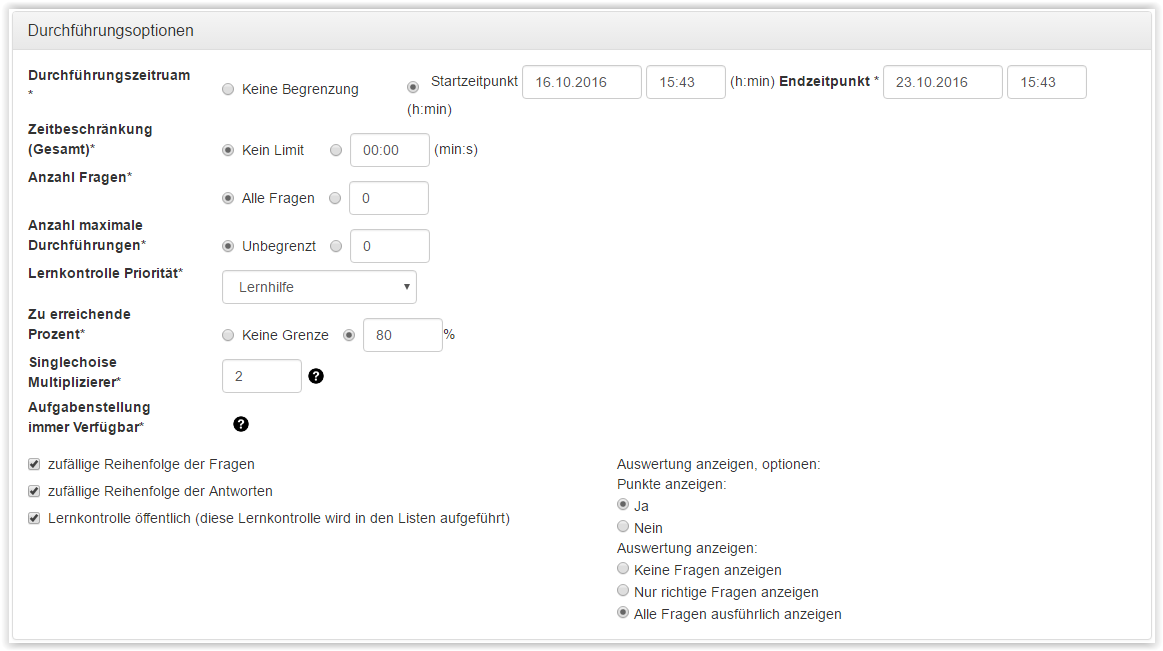
\includegraphics[width=0.75\textwidth
			]{Images/MobileQuiz_Quiz-Settings.PNG}
			\caption{Quiz-Einstellungen Mobile Quiz Version 3}
		\end{figure}
		
		
		Mobile Quiz bot zwar viele Einstellungsmöglichkeiten an, diese waren jedoch so zahlreich, dass sie den Benutzer fast überforderten. Zudem war die Darstellung zum Teil nicht optimal, da beispielsweise die 'Auswertung Anzeigen - Optionen' weiter rechts angezeigt wurde als alle anderen Einstellungen.
		
		\begin{figure}[H]
			\centering
			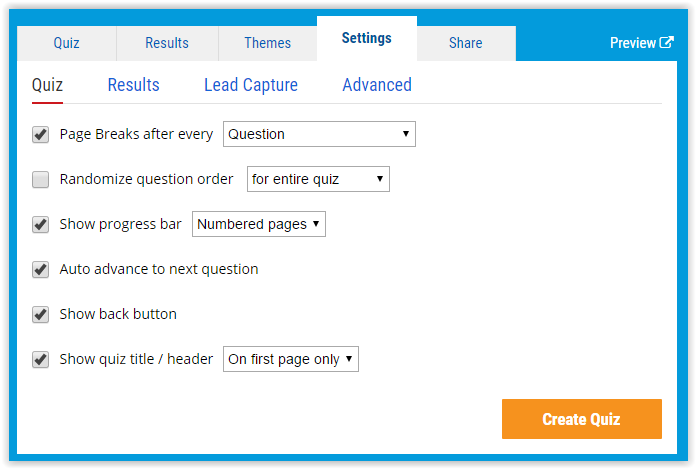
\includegraphics[width=0.5\textwidth
			]{Images/QuizMaker_Quiz-Settings.PNG}
			\caption{Quiz-Einstellungen Quiz Maker}
		\end{figure}
		
		Aufgeräumter wirkten die Einstellungen beispielsweise bei Quiz Maker \cite{quiz-maker}. Zwar gab es ebenfalls eine Vielzahl von Möglichkeiten, diese wurden aber übersichtlich dargestellt, indem sie Themen zugeordnet und auf Tabs verteilt wurden. Zudem gab es einen eigenen Tab für erweiterte Optionen. \\
		Bei Mobile Quiz waren beide Konzepte möglich, wodurch sich ein Quiz-Ersteller in den Einstellungen schneller zurechtfinden sollte.
		
		
		
		\item Quiz kann vor Veröffentlichung durchgespielt werden \\
		Wie sieht das erstellte Quiz für den Teilnehmer aus? Gibt es noch Rechtschreibfehler oder werden Inhalte nicht optimal dargestellt? Ein Quiz-Ersteller wird sich all diese Fragen womöglich stellen und die einfache Lösung dazu ist, dass man das Quiz vor Veröffentlichung selbst durchspielt. Die eigene Teilnahme soll jedoch nicht zählen, da sie die Auswertungsstatistik verfälschen kann. \\
		Mobile Quiz bot die Möglichkeit an, ein Quiz noch nicht zu veröffentlichen und es auf diese Weise auszuprobieren. Dies funktionierte aber nur, wenn man als Administrator eingeloggt war. Zudem zählte die eigene Teilnahme in die Gesamtauswertung mit hinein. Für die saubere Umsetzung musste also die Funktion für alle Ersteller-Rollen zugänglich sein und die eigene Teilnahme nicht mitzählen.
		
		
		
		\item Template für Frage-Import \\
		Ist man im Zug unterwegs und möchte trotzdem an einem neuen Quiz arbeiten, so fehlt meist der Internetzugang. Dies kompensierte Mobile Quiz dadurch, dass Fragen aus Excel-Dateien eingelesen und erstellt werden konnten. Um dies zu nutzen, benötigte es jedoch eine spezielle Formatierung, was neue Benutzer abschrecken konnte. \\
		Die Lösung dazu war es, ein Excel-Template, also eine Vorlage, für neue Fragen bereitzustellen. Darin kann der Benutzer schnell und einfach Fragen erfassen und muss sich nicht um das Format kümmern. Solche Templates bot beispielsweise
		Socrative \cite{socrative.com} an. Es ist im Anhang unter 'socrativeQuizTemplate.xlsx' zu finden.
		
		Im Rahmen dieser Arbeit wurde ebenfalls ein solches Template erstellt, welches nun Quiz-Erstellern zum Download angeboten wird.
		
	\end{itemize}	
	